% Created 2019-02-06 Wed 10:16
% Intended LaTeX compiler: pdflatex
\documentclass[10pt]{beamer}
\usepackage[utf8]{inputenc}
\usepackage[T1]{fontenc}
\usepackage{graphicx}
\usepackage{grffile}
\usepackage{longtable}
\usepackage{wrapfig}
\usepackage{rotating}
\usepackage[normalem]{ulem}
\usepackage{amsmath}
\usepackage{textcomp}
\usepackage{amssymb}
\usepackage{capt-of}
\usepackage{hyperref}
\usepackage{minted}
\usepackage{tikz}
\definecolor{cwiRed}{HTML}{BF1238}
\definecolor{cwiBlue}{HTML}{0B5D7D}
\setbeamertemplate{footline}[text line]{%
\parbox{\linewidth}{\noindent\vspace*{2pt}\noindent\rule{\linewidth}{0.4pt}\\{\scriptsize\noindent\vspace*{7pt}\insertshortauthor\hfill\insertshorttitle\hfill\insertdate}}
}
\renewcommand*\footnoterule{}
\usepackage{lmodern}
\usetheme[progressbar=head]{metropolis}
\author{Jan-Willem Buurlage}
\date{\today}
\title{Laboratory Class Scientific Computing WISM454, 2019}
\hypersetup{
 pdfauthor={Jan-Willem Buurlage},
 pdftitle={Laboratory Class Scientific Computing WISM454, 2019},
 pdfkeywords={},
 pdfsubject={},
 pdfcreator={Emacs 26.1 (Org mode 9.1.14)}, 
 pdflang={English}}
\begin{document}

\maketitle

\section{Organization}
\label{sec:orgb8c71dd}
\begin{frame}[label={sec:org4fcb14b}]{Expectations}
\begin{itemize}
\item Learn about \emph{random number generators}, \emph{Monte Carlo methods}, and \emph{genetic
algorithms}.
\item Develop \alert{scientific software} using C++.
\item Perform \alert{numerical experiments}.
\item Write \alert{coherent and concise reports}.
\item Reason about \alert{code performance}.
\end{itemize}
\end{frame}
\begin{frame}[label={sec:org57e8246}]{Grading}
\begin{itemize}
\item Hand-in assignments.
\item Two \(\pm 20\) page reports containing:
\begin{itemize}
\item Exercise solutions
\item Overview and explanation of code
\item Numerical experiments.
\end{itemize}
\item How the final grade is computed:
\begin{itemize}
\item \alert{\alert{Assignments:}} 20\%
\item \alert{\alert{Report I:}} 40\%
\item \alert{\alert{Report II:}} 40\%
\end{itemize}
\item The focus of the course is on developing your programming skills, and writing
good reports.
\end{itemize}
\end{frame}
\begin{frame}[label={sec:org499dbee}]{Topics}
\begin{itemize}
\item \alert{Randomized algorithms and tools}
\begin{enumerate}
\item Random number generation
\item Monte Carlo methods
\item Genetic algorithms
\end{enumerate}
\item Introduction to C++, for developing \alert{high-performance code}
\item Software engineering skills, software architecture, \alert{scientific programming}
\end{itemize}
\end{frame}
\section{Random number generators}
\label{sec:org2573c46}
\begin{frame}[label={sec:org39bf316}]{RNGs}
\begin{itemize}
\item Random number generator (RNG): \alert{A means to get uniformly distributed numbers.}
\item We focus on obtaining numbers in the set:
$$M = \{ 0, 1, \ldots, m - 1 \}.$$
\item An RNG can be a physical device, process, or a algorithm.
\end{itemize}
\end{frame}
\begin{frame}[label={sec:org8437069}]{Pseudo RNGs}
\begin{itemize}
\item For scientific computing, we value the following properties in our RNG
\begin{itemize}
\item \alert{Randomness}
\item \alert{Reproducibility}
\item \alert{Efficiency}
\end{itemize}
\item We focus on computer based RNGs, which are deterministic.
\item Deterministic seems paradoxical, usually called pseudo-RNGs (PRNGs).
\end{itemize}
\end{frame}
\begin{frame}[label={sec:org829aab9}]{Iterations}
\begin{itemize}
\item Classic PRNGs have the form:
$$x_{i + 1} = f(x_i).$$
The next iterate of a sequence of random numbers produced by PRNGs of this form depend completely on the previous iterate.
\item We start the sequence by choosing an initial number \(x_0\). This is called the \alert{seed}.
\item If you use the same seed, you get the same sequence \(\implies\) reproducible.
\end{itemize}
\end{frame}
\begin{frame}[label={sec:org8a657c7}]{Real numbers}
\begin{itemize}
\item Say we want numbers not in \(M\) but in \([0, 1]\). We can scale:
\end{itemize}
$$\omega_i \equiv \frac{x_i}{m - 1}.$$

\begin{itemize}
\item \uline{Ex. 2.1}: or should we scale in another way?
\item The usual strategy is to have an \alert{engine} that generates integers uniformly. Using these
random integers, other \alert{distributions} can be realized.
\end{itemize}
\end{frame}
\begin{frame}[label={sec:org055eaf8}]{Linear congruential RNG}
\begin{itemize}
\item The \alert{linear congruential RNG} (LCRNG) has the following form for \(f\):
$$f(x) = (a x + c) \bmod m.$$
\item Here, \(a\), \(c\), and \(m\) are integer parameters that define the LCRNG.
\item Easy to implement, but have some drawbacks.
\end{itemize}
\end{frame}
\begin{frame}[label={sec:org95cf343}]{Example:}
\begin{itemize}
\item Let us choose: \(a = 5, c = 2, m = 6, x_0 = 3\)
\item \((5 \times 3 + 2) \bmod 6 = 5\)
\item And then the next element in the sequence is \ldots{} again \(3\)
\item Although there are \(m\) possible output numbers, we can have \alert{repeating cycles}
like here (3, 5, 3, 5, 3, 5, \ldots{}).

\item (Question: should we include the seed in the sequence?)
\end{itemize}
\end{frame}

\begin{frame}[label={sec:org65623e2}]{Period of LCRNG}
\begin{definition}
The smallest $n$ such that $x_{i + n} = x_i$ is called the period of the LCRNG. If $n = m$, then full period.
\end{definition}

\begin{itemize}
\item \uline{Ex 2.2}: what if \(c = 0\)?

\item Full period means that the LCRNG gives a permutation of \(M\).

\item \emph{True} uniform distributions would likely produce the same numbers \alert{multiple
times without repeating}.

\item Numbers may become very large. We want to use the maximum \(m\) that we can
\alert{still represent efficiently on the computer}.
\end{itemize}
\end{frame}
\begin{frame}[label={sec:org147ad73}]{Binary numbers on computers}
\begin{itemize}
\item Unsigned integers are typically stored in 32 bits (= 4 bytes) or 64 bits.
\end{itemize}
$$x = \sum_{i = 0}^{n - 1} b_i 2^i.$$
\begin{itemize}
\item Some examples:
\begin{align*}
2 &= 10_2 \\
5 &= 101_2 \\
23 &= 10111_2
\end{align*}
\item Least significant (right), most significant (left).
\item Addition throws away most significant bits (overflow). \alert{Arithmetic operations
on \(n\text{-bit}\) integers are like working modulo \(2^n\)}!
\end{itemize}
\end{frame}
\begin{frame}[label={sec:org435786a}]{Negative numbers}
\begin{itemize}
\item Signed integers. Most significant bit is the \alert{sign bit}.
\item If the sign bit is 0 then the number is positive, if it is 1 then it is
negative.
\item However, it is done in a smart way called \alert{two's complement encoding}!
Corresponding to the following sequence:
\end{itemize}
$$\{ 0, \ldots (2^{n-1} - 1), -2^{n-1}, \ldots, -1 \}.$$
\end{frame}
\begin{frame}[label={sec:org3655398}]{Two's complement encoding.}
\begin{itemize}
\item Signed versus unsigned:
$$(-a)_\text{s} \equiv (2^n - a)_{\text{u}}$$
\item \alert{Note:} \(2^n - a \equiv (2^n - 1) - a + 1\), so in \alert{summary}: \(-a\): invert all
bits of \(a\) and add \(1\).
\item Subtraction can then be implemented by addition.
\begin{align*}
(x + (-y)_{\text{u}}) \bmod 2^n &= (x + 2^n - 1 - y + 1) \bmod 2^n\\
&= (x - y) \bmod 2^n.
\end{align*}
\end{itemize}
\end{frame}
\begin{frame}[label={sec:org846e110}]{Shrage's trick}
\begin{itemize}
\item Now that we are a bit familiar with binary representation of numbers on computers, we consider possible issues.
\end{itemize}

\uline{Ex 2.4}: \(m = 2^b, c \neq 0 \implies\) not random in all bits

\begin{itemize}
\item For this reason, we want \(m = p\) prime, if \(c = 0\):
$$f(x) = ax \bmod m.$$
However, what if \(ax\) \alert{overflows}?
\item If we could factorize \(m = aq\) then:
$$ax \bmod m = ax \bmod aq = a (x \bmod q).$$
(note that this is always smaller then \(m\))
\end{itemize}
\end{frame}
\begin{frame}[label={sec:org289aeda}]{Shrage's trick (II)}
\begin{itemize}
\item However, we would like \(m\) prime\ldots{}
\item Assume \(m = aq + r\) with \(r\) small, then (try to prove this for your report):
\begin{align*}
b \equiv a (x \bmod q) - r (x~\text{div}~q) \\
ax \bmod m = \begin{cases}
b & \text{ if } b \geq 0 \\
b + m & \text{otherwise}
\end{cases}
\end{align*}
and if \(r < q\) all numbers involved are less than \(m\), so we can compute without overflow.
\item This is called \alert{Shrage's trick}
\end{itemize}
\end{frame}

\begin{frame}[label={sec:org281f3fd}]{Summary}
\begin{itemize}
\item An \alert{RNG engine} generates numbers in the set:
$$M = \{0, 1, \ldots, m - 1\}.$$
\item For \alert{scientific experiments}, we want reproducibility, efficiency and
randomness.
\item \alert{LCRNGs} are simple generators that can generate pseudo-random
sequences.
\item Correct implementations require you to be aware of how integers are \alert{encoded} in
your computer.
\end{itemize}
\end{frame}
\section{C++}
\label{sec:org28a0a2e}
\begin{frame}[label={sec:org5bcbf13}]{C++}
\begin{itemize}
\item Compiled language!
\begin{itemize}
\item \emph{source(s)} \(\to\) \alert{\uline{compile}} \(\to\) \emph{object file(s)} \(\to\) \alert{\uline{link}} \(\to\) \emph{single executable}
\end{itemize}
\item Source code is portable, but the executable generally is not (contrary to e.g. Java)
\item \alert{Language features}
\begin{itemize}
\item types, functions, control flow statements
\end{itemize}
\item \alert{Standard library}
\begin{itemize}
\item containers, IO operations, \ldots{}
\item implemented using language features (could build this yourself on top of C++!)
\end{itemize}
\end{itemize}
\end{frame}
\begin{frame}[fragile,label={sec:org7d46256}]{Smallest C++ program}
 \begin{minted}[frame=none,xleftmargin=\parindent]{cpp}
int main() { return 0; }
\end{minted}

\begin{itemize}
\item The \texttt{main} function is called when the C++ program is executed. One main function across all your source files!

\item \texttt{int main() \{\}} is actually also a valid C++ program
\end{itemize}
\end{frame}
\begin{frame}[fragile,label={sec:orgaa22d8a}]{Output}
 \begin{minted}[frame=none,xleftmargin=\parindent]{cpp}
#include <iostream>

int main() {
    // console out
    // read << as 'put to'
    // std is a namespace
    std::cout << "Hello, world!\n";
}
\end{minted}

Note: \alert{semicolon} ;
\end{frame}

\begin{frame}[fragile,label={sec:org091f275}]{Types}
 Every entity has a type, which determines what is valid for that entity. Types are used e.g. to denote the type of the return value of a function (as in main), or its parameters.

\begin{minted}[frame=none,xleftmargin=\parindent]{cpp}
int square(int x) {
    return x;
}

...

std::cout << square(3) << "\n";
\end{minted}
\end{frame}

\begin{frame}[fragile,label={sec:orgfc444f9}]{Built-in types}
 There are a number of 'fundamental' (not user-defined) types.

\begin{itemize}
\item \texttt{bool} (1)
\item \texttt{char} (1)
\item \texttt{int} (4)
\item \texttt{double} (8)
\end{itemize}

\begin{minted}[frame=none,xleftmargin=\parindent]{cpp}
int x = 3;
int z = x + 5; // FINE!
bool a = false;
bool b = a + 3; // ERROR!
\end{minted}
\end{frame}

\begin{frame}[fragile,label={sec:org6d660fa}]{Caveats}
 \begin{minted}[frame=none,xleftmargin=\parindent]{cpp}
int b = 7.1; // no error!
float a = 3.0;
float a = 312489012480918240.0;
float a = 3124.0f;
\end{minted}
\end{frame}
\begin{frame}[fragile,label={sec:org0709923}]{Narrowing}
 Lenient with conversions (narrowing!), can be dangerous. C++11:
\begin{minted}[frame=none,xleftmargin=\parindent]{cpp}
int b{7.1}; // error!
float a{3.0} // error!
auto a = 12345.0; // a is a double!
\end{minted}
(I generally use \texttt{auto} everywhere, and if necessary annotate on the right).

Some useful operations:
\begin{minted}[frame=none,xleftmargin=\parindent]{cpp}
x += y; // - * / %
++x;
x++;
\end{minted}
\end{frame}
\begin{frame}[fragile,label={sec:orgbcc8f6e}]{Constants}
 \begin{minted}[frame=none,xleftmargin=\parindent]{cpp}
const auto x = 3;
x = 5; // ERROR!
\end{minted}
\end{frame}
\begin{frame}[fragile,label={sec:org0991faf}]{Control flow statements}
 \begin{minted}[frame=none,xleftmargin=\parindent]{cpp}
int x = 2;

if (x > 3) {
    f();
} else {
    g();
}

while (x < 3) {
    x += 1;
}
\end{minted}
\end{frame}
\begin{frame}[fragile,label={sec:org6afe87d}]{For loop}
 \begin{minted}[frame=none,xleftmargin=\parindent]{cpp}

// this
for (int i = 0; i < 5; ++i) {
    std::cout << i << "\n";
}
// is equivalent to
int i = 0;
while (i < 5) {
    std::cout << i << "\n";

    ++i;
}
\end{minted}
\end{frame}

\begin{frame}[fragile,label={sec:org4cc1bcd}]{Pointers, arrays}
 \begin{minted}[frame=none,xleftmargin=\parindent]{cpp}
int xs[6] = {0, 1, 2, 3, 4, 5}; // array of ints
int* ys = nullptr; // pointer to int
int* x = &x[3]; // address of 4th element
int y = *x; // y = contents of x
\end{minted}
\end{frame}
\begin{frame}[fragile,label={sec:orgef60fa1}]{Structures}
 \begin{minted}[frame=none,xleftmargin=\parindent]{cpp}
struct lcrng {
    int a;
    int c;
    int m;
};
\end{minted}

\begin{itemize}
\item \alert{User defined type}!
\end{itemize}

\begin{minted}[frame=none,xleftmargin=\parindent]{cpp}
int next(lcrng generator, int x) {
    // ... (generator.a)
}
\end{minted}
\end{frame}

\begin{frame}[label={sec:org60c86ad}]{Programming environment}
\begin{center}
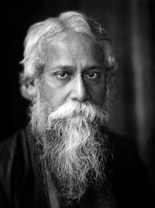
\includegraphics[width=100px]{./tagore.jpg}
\end{center}

\begin{QUOTATION}
“I have spent many days stringing and unstringing my instrument 
while the song I came to sing remains unsung.”

― \emph{Rabindranath Tagore}
\end{QUOTATION}
\end{frame}
\begin{frame}[label={sec:org547dc8e}]{Programming environment (II)}
\begin{center}
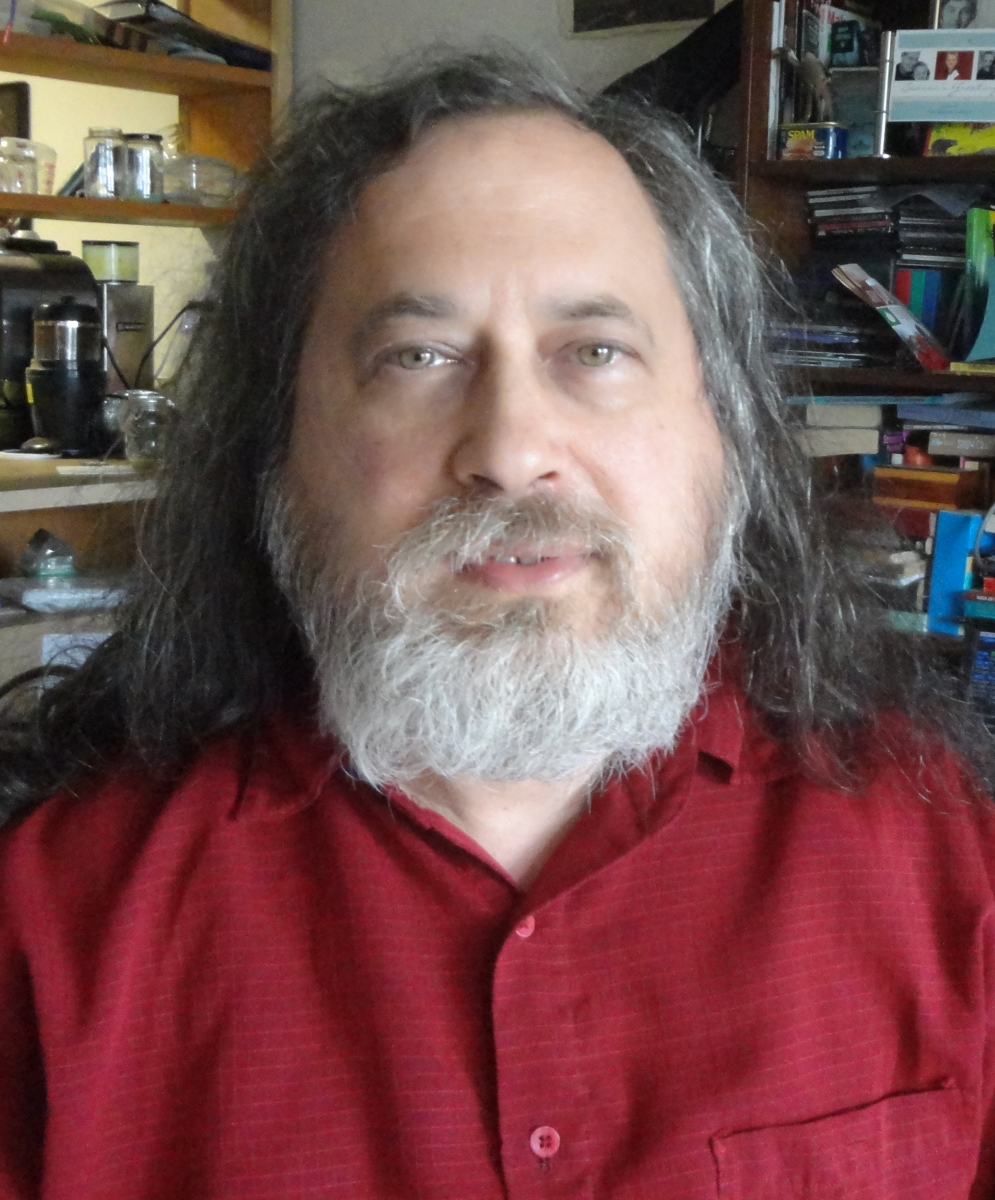
\includegraphics[width=100px]{./stallman.jpg}
\end{center}

\begin{QUOTATION}
“Sharing is good, and with digital technology sharing is easy.”

― \emph{Richard Stallman}, founder of GNU
\end{QUOTATION}
\end{frame}
\begin{frame}[label={sec:org0a61e72}]{Minimal C++ programming environment}
\begin{itemize}
\item \emph{Windows}
\begin{itemize}
\item \alert{Notepad++} and \alert{CygWin}
\end{itemize}
\item \emph{Linux}
\begin{itemize}
\item \alert{gedit} and \alert{GCC}
\end{itemize}
\item Your code must be written in \emph{standard C++}, and be buildable with a common
cross-platform build tool (more on this in the upcoming weeks).
\end{itemize}
\end{frame}
\begin{frame}[label={sec:org455ab53}]{This week}
\begin{itemize}
\item Set up programming environment
\item Compile and run ``Hello, world!''
\item Write a simple LCRNG function
\item Exercises \alert{2.1, 2.2}
\item Exercise \alert{2.6}: implement and experiment with a number of RNGs (Note: course
website linked to in LNs is outdated)
\end{itemize}
\end{frame}
\end{document}